
\chapter{Metodologia} \label{cap:metodos}


% ISSO aqui é metodologia
%Como foi evidenciado nas comunicações com a gestão do restaurante, a análise utilizada para se prever as refeições é produzir no dia da semana, como por exemplo uma segunda-feira, o consumo do mesmo dia da semana anterior (segunda-feira anterior) com acréscimo de uma margem de erro. Em geral, de acordo com o restaurante, todos os dias o mesmo trabalha com um erro e um descarte de 30\% das refeições que são trazidas e consumidas ao campus. Estima-se então que no período de 2011 - 01/08/2018 os estabelecimentos tenham tido um prejuízo de R\$1.885.938,40, e de 30\% de R\$78.386,85 no atual período de 01/08/2018 - 31/10/2018 totalizando o montante  R\$1.964.325,25. Aproximadamente 2 milhões de reais em prejuízo acumulado desde 2011.



% A obtenção dos dados do R.U do ICT Unifesp se encontra em formato de série temporal, ou seja, o consumo e vendas de refeições no R.U se distribuem em função do tempo, pelos dias letivos da universidade.
 
 
 % O cenário deste estudo analisa a sazonalidade da frequência de alunos do ICT - UNIFESP, inferida pelas grades semestrais de suas disciplinas, que consequentemente inferem na sazonalidade de consumo de refeições dentro do restaurante universitário. 
 
 
 
 
   Neste Capítulo é descrita a metodologia experimental deste trabalho, a qual consiste nos seguintes passos:
    \begin{itemize}
        \item Coleta de dados endógenos e exógenos.
        \item Transformação de cada registro de dado endógeno (os dados de consumo e vendas), em uma série temporal com intervalo de cinco dias anteriores.
        \item Análises exploratórias dos conjuntos de dados endógenos e exógenos com o conjunto de dados a serem previstos.
        \item Construção e treino dos modelos exclusivamente endógenos e dos modelos mistos, duplicados em duas fases experimentais com diferentes domínios temporais.
        \item Análises comparativas dos resultados dos modelos.
    \end{itemize}
    
    \section{Área de estudo}
       A área de estudo deste trabalho é o restaurante universitário do Instituto de Ciência e Tecnologia da Unifesp (ICT-Unifesp) em São José dos Campos. O campus do ICT foi inaugurado no ano de 2007 visando suprir as demandas científicas e tecnológicas da região do Vale do Paraíba. A Figura \ref{fig:RU_foto} apresenta um dia comum de utilização do espaço físico do restaurante unuversitário do ICT.
        
        \begin{figure}[H]
        	\center{
        	    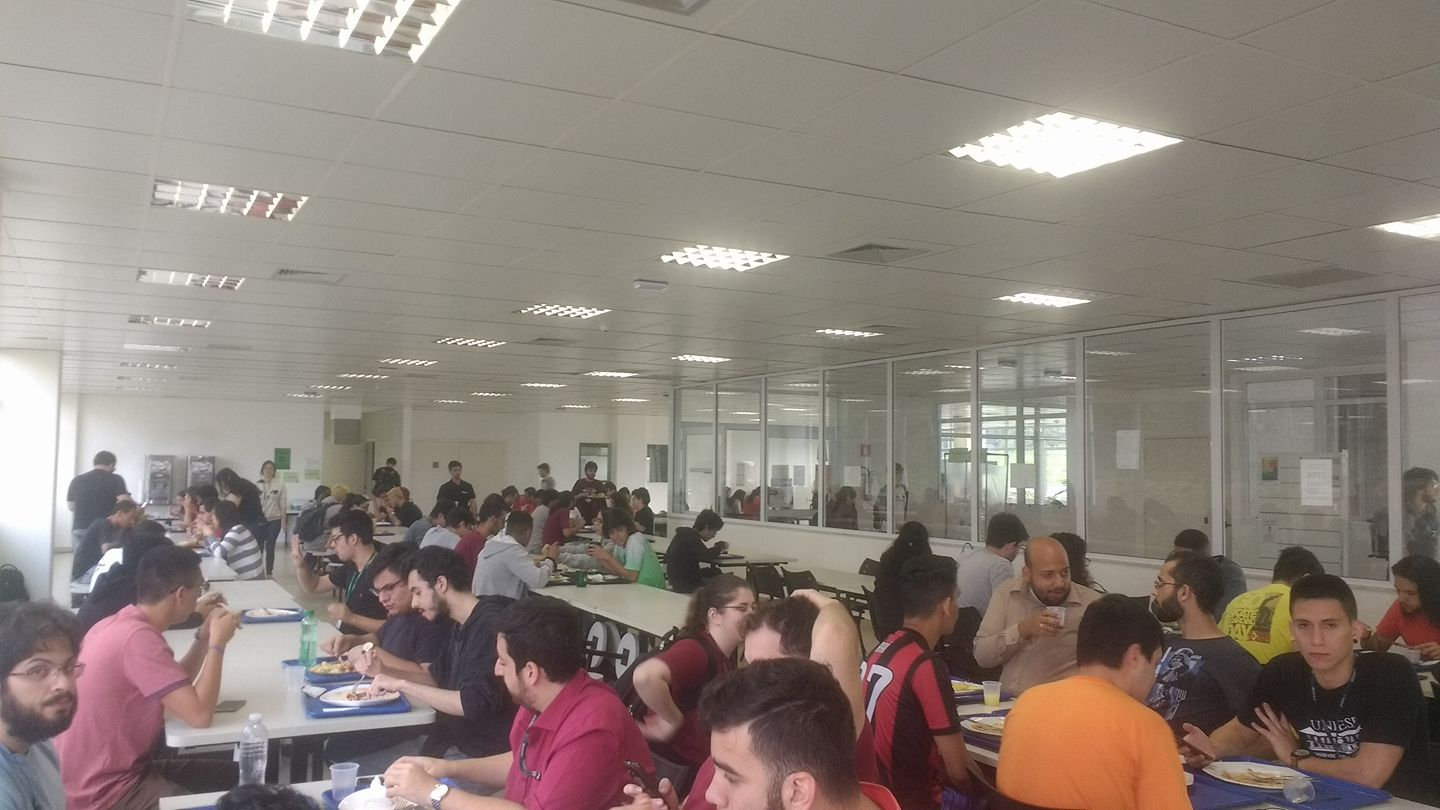
\includegraphics[width=0.7\textwidth]{./Figuras/ru_unifesp.jpg}
        	    \caption{Restaurante Universitário do ICT-Unifesp}\label{fig:RU_foto}
        	     }
        \end{figure}
    
    \section{Descrição dos dados}

    Este trabalho fará uso de dois tipos de dados, endógenos e exógenos, os quais são descritos a seguir. 
            
    Dados endógenos:  são os dados do domínio de predição neste caso. Para este problema, são as quantidades diárias de  refeições consumidas no almoço e no jantar do Restaurante Universitário (RU) do ICT-Unifesp, quantificada diariamente pela número de alunos que passam no ponto de acesso, a catraca. 
    Também são considerados dados endógenos a quantidade diária  de \textit{tickets} de refeição vendidos pelo Restaurante. Em ambos casos, as informações são tidas dos dias letivos.   Esses dados são transformados em entrada de redes neurais, em formato de série temporais.
            
    Dados exógenos: são todos os outros dados fora do domínio de predição. Para este problema, são  parâmetros derivados das datas das observações, como por exemplo o dado categórico que representa o dia da semana (segunda-feira à sexta feira), e os dados climáticos.
    
    \section{Obtenção e tratamento dos dados}
        A obtenção dos dados é realizada por meio de duas fontes distintas, sendo os dados endógenos inteiramente fornecidos através do setor de tecnologia da informação do ICT Unifesp, parte dos dados exógenos da data de registro dos dados endógenos coletados, e a parte restante dos dados exógenos, os dados climáticos, são obtidos através da uma estação meteorológica mais próxima ao ICT Unifesp, localizada na cidade de Taubaté-SP.
        
	    \subsection{Dados endógenos} \label{subsec:coleta_endogenos}
        	Os dados históricos de consumo no restaurante foram retirados do atual sistema banco de dados de refeições subsidiadas do Hospital São Paulo, que gerencia os dados dos refeitórios de todos as unidades da Unifesp. Apenas alguns funcionários autorizados têm acesso ao banco de dados da instituição, portanto para coletar tais dados o presente trabalho obteve uma autorização com a direção do campus ICT-Unifesp. Foram solicitados  os dados de consumo apenas para os discentes de graduação, visto que  o banco de dados ainda possui as informações de consumo de docentes, alunos de pós-graduação e visitantes, porém claro com menor relevância em termos quantitativo. Além disso, o padrão de consumo destes outros estratos do meio acadêmico pode influenciar  o processo de predição das demandas trazendo tendências diferentes. Na tabel \ref{table:dadosrestaurante}.
    
        	\begin{table}[!ht]
        	    \centering
        	    \caption{Formato original dos dados originais obtidos pelo restaurante universitário}
                \rowcolors{2}{gray!25}{white}
                \begin{tabular}{l|l|l}
                    \hline
                    DATA                  & (19/12/2017) & (18/12/2017) \\ \hline
                    VENDAS CAFÉ           & 0            & 0            \\
                    VENDAS ALMOÇO         & 24           & 71           \\
                    VENDAS JANTAR         & 0            & 0            \\
                    VENDAS REFEIÇÃO      & 24           & 71           \\
                    TOTAL VENDAS          & 24           & 71           \\
                    ENTR. CAFÉ            & 0            & 0            \\
                    ENTR. ALMOÇO          & 42           & 70           \\
                    ENTR. JANTAR          & 3            & 24           \\
                    TOTAL ENTR. REFEIÇÃO & 45           & 94           \\
                    TOTAL ENTRADA         & 45           & 94           \\ \hline
                \end{tabular}
               
                \label{table:dadosrestaurante}
            \end{table}
            
            Após a coleta, os dados de consumo do restaurante foram transformados em um processo de aproximação por uma série temporal, para um intervalo de cinco dias, e em cada registro de venda  acrescentados cinco novos atributos contendo os valores passados, deste mesmo atributo, em um intervalo de cinco dias anteriores. Este processo adapta o conjunto de dados para o processo de memorização das entradas, estruturando o formato compatível de leitura de dados nos modelos de redes neurais aplicados.
            
            A Tabela \ref{table:transformacaodadosrestaurante} exemplifica a nova estrutura de um registro de dado do restaurante, com um intervalo temporal de cinco dias anteriores. Nota-se que o valor de consumo da data 20/04/2017 foi removido do conjunto de dados, por se tratar o valor supervisionado a ser previsto, dado que o processo de aprendizado das redes neurais utilizam apenas dados no passado, a partir de um dia anterior.
            
            \begin{table}[!ht]
                \centering
                \rowcolors{2}{gray!25}{white}
                \begin{tabular}{l|l}
                \hline
                    DATA                  & (19/12/2017) \\ \hline
                1 DIA ANTERIOR    & 500        \\
                2 DIAS ANTERIORES & 00                            \\
                3 DIAS ANTERIORES & 300                            \\
                4 DIAS ANTERIORES & 200                            \\
                5 DIAS ANTERIORES & 100                          \\ \hline 
                \end{tabular}
                \caption{Transformação dos registros do restaurante em uma série temporal.}
                \label{table:transformacaodadosrestaurante}
            \end{table}
           
        \subsection{Dados exógenos} \label{subsec:coleta_exógenos}
            Os dados exógenos correlacionados com o consumo se dividem em dois tipos principais, dados climáticos coletados de estações meteorológicas próximas ao ICT-Unifesp, e dados derivados das datas dos registros de consumo.
    
      	 Em relação as variáveis climáticas utilizadas como dados exógenos, foram considerados parâmetros que possam afetar o consumo de refeições de forma indireta, como temperatura média ambiente, pressão atmosférica, umidade e velocidade do vento. Tais parâmetros podem ser obtidos de forma gratuita pelo BDMEP - Banco de Dados Meteorológicos para Ensino e Pesquisa, pertencente à instituição pública INMET - Instituto Nacional de Meteorologia, pertencente ao Ministério da agricultura, pecuária e abastecimento. É necessário um cadastro na plataforma do INMET \footnote{\url{http://www.inmet.gov.br/portal/index.php?r=bdmep/bdmep}} para a obtenção dos dados. A instituição contêm dados registrados de forma digital desde 1961 no país inteiro, os dados históricos referentes a períodos anteriores a 1961 ainda não estão em forma digital e, portanto, estão indisponíveis no BDMEP. Importante ressaltar que o BDMEP leva 90 dias para registrar cada nova data. 
            	
     	  Além dos dados ambientais, também foram gerados dados exógenos a partir dos dados de consumo coletados. A informação de data contida nos índices dos registros dos dados endógenos, foi derivada em diversas informações que representam o comportamento de consumo em relação à sazonalidade da frequência dos alunos influenciada pelas agendas de atividades acadêmicas.\\
            	Os seguintes parâmetros foram definidos:
            	\begin{itemize}
            	    \item Semestre 1 ou 2 em formato categórico e binário;
            	    \item Dia da semana em formato categórico e binário;
            	    \item Distancia em dias até o registro anterior e posterior;
            	    \item Avanço do semestre em escala percentual;
            	    \item Avanço do mês em escala percentual.
            	\end{itemize}
            	
            	O consumo distribuído em uma janela de cinco dias para entrada nas redes MLP seguiu padrão semelhante com os trabalho de previsão de demanda em R.U realizados por \citeonline{Lopes2008} e \citeonline{Rocha2011}, ilustrado na Figura \ref{fig:mlp-lopes}. Por fim, a Tabela \ref{table:dataset_final} representa o conjunto de dados estruturados e preparados para o processo de divisão em domínios de treino, validação e teste para o treino dos modelos.

       \begin{table}[!ht]
            \centering
            \rowcolors{2}{gray!25}{white}
            \begin{tabular}{c|c|c} \hline
                \multicolumn{3}{c}{ Estrutura final do conjunto de dados indexados por data: } \\
                \hline
                identificador &	nome da variável					&tipo de variável\\ 
                \hline
                0&	SEMESTRE\_1					&int64 \\
                1&	SEMESTRE\_2					&int64\\
                2&	SEGUNDA						&int64 \\
                3&	TERCA						&int64 \\
                4&	QUARTA						&int64 \\ 
                5&	QUINTA						&int64 \\ 
                6&	SEXTA						&int64 \\ 
                7&	DISTANCIA\_DIA\_ANTERIOR	&	int64 \\ 
                8&	DISTANCIA\_DIA\_POSTERIOR	&	int64 \\
                9&	PERC\_CONCLUSAO\_SEM		&	float64 \\
                10&	PERC\_CONCLUSAO\_MES		&	float64 \\
                11&	PRESSAO\_ATMOSFERICA		&	float64 \\
                12&	TEMPERATURA					&float64 \\ 
                13&	UMIDADE						&int64 \\
                14&	VENTO						&float64\\ 
                15&	VENDAS\_ALMOCO				&int64 \\
                16&	VENDAS\_ALMOCO\_1			&	int64 \\ 
                17&	VENDAS\_ALMOCO\_2			&	int64 \\
                18&	VENDAS\_ALMOCO\_3			&	int64\\ 
                19&	VENDAS\_ALMOCO\_4			&	int64 \\
                20&	VENDAS\_ALMOCO\_5			&	int64 \\ 
                21&	ENTR\_ALMOCO				&	int64\\
                22&	ENTR\_ALMOCO\_1				&int64 \\
                23&	ENTR\_ALMOCO\_2				&int64 \\
                24&	ENTR\_ALMOCO\_3				&int64 \\ 
                25&	ENTR\_ALMOCO\_4				&int64 \\
                26&	ENTR\_ALMOCO\_5				&int64 \\
                27&	ENTR\_JANTAR				&	int64 \\ 
                28&	ENTR\_JANTAR\_1				&int64\\
                29&	ENTR\_JANTAR\_2				&int64 \\ 
                30&	ENTR\_JANTAR\_3				&int64 \\ 
                31&	ENTR\_JANTAR\_4				&int64 \\
                32&	ENTR\_JANTAR\_5				&int64\\
              \hline
            \end{tabular}
            \caption{Estrutura final do conjunto de dados indexados por data}
            \label{table:dataset_final}
        \end{table}
        Por fim, a Tabela \ref{table:dataset_final} representa o conjunto de dados estruturados e preparados para o processo de divisão em domínios de treino, validação e teste para o treino dos modelos.
        
	\subsection{Pré-processamento}
        Na etapa de pré-processamento é realizada a transformação dos dados endógenos em séries temporais, de comprimento de cinco dias, normalização com remoção de \textit{outliers}, e aplicação de escala 0 a 1, para que todos os dados correspondam à um mesmo domínio de aprendizado. Após a conclusão destas etapas, o conjunto de dados foi preparado para as fases experimentais 1 e 2, que realizaram uma divisão do conjunto final de dados em intervalos temporais distintos. Apesar da distribuição dos dados se apresentarem em datas em função do tempo se classificando em um modelo de série temporal, assume-se a hipótese que o comportamento dos mesmos também é impactado por relações causais com outros variáveis exógenas, como recesso acadêmico, feriados, eventos, precipitações intensas que causam trânsito local e impactam na logística e frequência do público, entre outras variáveis de causas menos aparentes
    
        \subsection{Tratamento dos dados para entrada nos modelos}
         	Os dados endógenos, após estruturados na tabela final do conjuntos de dados, passam pelas seguintes transformações:
         	\begin{itemize}
                \item	Calculo do desvio padrão de cada vetor de atributos, e normalização dos valores máximos para o teto de 3x o desvio padrão, e mínimo de 0; 
                \item	Transformação dos dados em escala de 0 e 1.
            \end{itemize}
            Os dados exógenos não passam pela transformação em série temporal, portanto os mesmos foram tratados de acordo com os passos:
            \begin{itemize}
                \item	Transformação dos dados em escala de 0 e 1;
                \item	Os parâmetros categóricos binários (dias da semana e semestre) já estão escalados por serem categorias binárias.
            \end{itemize}
    	\subsection{Fases Experimentais} \label{subsec:fases_experimentais}
            O processo experimental foi realizado em dois roteiros distintos de divisão do domínio temporal do conjunto de dados, e os resultados obtidos entre as duas fases foram comparados.
            
            O conjunto de dados contemplando o período de 2017 a 2019, foi dividido em conjunto de treino, validação e teste da seguinte maneira: 
            
            \paragraph{1º Fase com validação no 1º semestre de 2018 e teste no 1º semestre de 2019}
                Neste roteiro, o semestre de validação que compõe o conjunto de dados para o treino \textit{backpropagation} das redes neurais contempla o primeiro semestre de 2018 e o conjunto de teste contempla o primeiro semestre de 2019.
                Os dados de 2017 contemplando o 1º e 2º semestre, e 2018 contemplando o 2º semestre, foram usados para treino. Os resultados obtidos nesta divisão foram usados para validar a hipótese de que os modelos aprendem especificamente a sazonalidade de consumo no primeiro semestre, se saindo melhor nos testes realizados no primeiro semestre de 2019, em comparação aos outros modelos treinados com validação no ano todo de 2018.
                Portanto, o conjunto de dados da primeira fase contempla o seguinte domínio:
            \begin{itemize}
                    \item Conjunto de treino dos modelos, contemplando o primeiro e segundo semestre de 2017, e segundo semestre de 2018;
                    \item Conjunto de validação dos modelos, contemplando o primeiro semestre de 2018;
                    \item Conjunto de teste dos modelos, contemplando o primeiro semestre de 2019.             
            \end{itemize}
            
            \paragraph{2º Fase com treino em 2017, validação em 2018 e teste em 2019}
                Nesta fase, os conjuntos foram divididos conforme sua descrição e o melhor modelo encontrado passa por uma última etapa de teste no domínio da primeira fase (teste somente no primeiro semestre de 2019).
                As métricas obtidas neste teste foram comparadas com o melhor modelo da primeira fase.
    
    \section{Definição e treino dos modelos}
            %\paragraph*{Sobre a necessidade de implementar modelos mistos}
                No conjunto de dados deste trabalho, os dados obtidos se dividem em dados temporais e endógenos (tal que cada registro de consumo e venda trás a informação de seu domínio em um intervalo temporal de cinco dias anteriores) e dados discretos e exógenos, sendo variáveis categóricas de data para cada registro, e variáveis climáticas.
                
                Portanto foi necessária a implementação de modelos específicos para entradas temporais e modelos específicos para as entradas discretas.
                Para a saída final foi implementado um comitê de redes neurais endógenas e exógenas, com um neurônio perceptron na saída, recebendo os dois valores dos modelos endógenos e exógenos para a regressão das saídas das duas redes ao valor que será a predição do consumo.
         	\paragraph{Modelos endógenos}
         	\begin{itemize}
                \item	Desenvolvimento das redes perceptron de baixa profundidade para avaliar o aprendizado da rede;
                \item	Aumento da profundidade da rede e avaliar as mudanças da função de perda RMSE; 
                \item	Implementação e avaliação dos modelos com redes recorrentes GRU, conforme a Figura. \ref{fig:gru-arch} que são especialmente desenvolvidos para o aprendizado com memorização de dados, e no caso deste trabalho, podem memorizar as sazonalidades semanais de consumo (em um intervalo de cinco dias).
            \end{itemize}
            \paragraph{Modelos Mistos : Endógenos e Exógenos}
                \begin{itemize}
                    \item Para os dados temporais (consumo e venda) utilizou-se os melhores modelos endógenos dos experimentos anteriores para as entradas endógenas. 
                    \item Para os dados discretos e categóricos adaptou-se a entrada destes dados para rede perceptron
                    \item  Concatenou-se a saída das duas redes neurais em um perceptron criando um comitê de redes neurais para obter a saída final prevista.
                \end{itemize}
            
	\subsection{Hiper parâmetros : Função de ativação e otimizador}
        Conforme fundamentado no Capítulo \ref{cap:teoria} na Seção \ref{sec: perceptron}, a função de ativação dá a capacidade do perceptron, quando conectado em rede, de resolver problemas lineares e não lineares, agregando adaptação e improviso ao resolver programas que não estão contidos em seus dados de alimentação.
        Portanto para as camadas ocultados das redes neurais MLP desenvolvidas será aplicada a função ReLu e para o neurônio de saída será aplicada a função linear, e o otimizador de treino realiza a função de otimizar o tempo de convergência do reajuste dos pesos à valores ideais, sendo escolhido o otimizador ADAM com taxa de aprendizado definido em 0,001.

    \section{Teste e Métricas de avaliação}
       As principais métricas de avaliação dos modelos são a Raiz do Erro Quadrático Médio ou em inglês \textit{Root Mean Squared Error} (RMSE), O coeficiente de correlação de Pearson (R), e o coeficiente "chi-quadrado" definido como $R^2$. Estas métricas estatísticas foram utilizado nas etapas de teste para avaliar a proximidade das predições do modelo com o comportamento real de consumo. As equações \ref{eq:RMSE} e \ref{eq:Pearson} apresentam a formulação para o RMSE e o coeficiente de Pearson (R), respectivamente.
       
       \begin{equation}
           RMSE = \sqrt{\frac{1}{n}  \sum_{i=1}^n (x_i^{est} - x_i^{obs})^2}
           \label{eq:RMSE}
       \end{equation}
       
       \begin{equation}
           R = \frac{\frac{1}{n}  \sum_{i=1}^n (x_{est} - \bar{x}_{est}) * (x_{obs} - \bar{x}_{obs})}{\sigma_{est} * \sigma_{obs} }
           \label{eq:Pearson}
       \end{equation}
       
       Onde “est” são os valores estimados; “obs” são os valores reais; n é o numero de amostras ; $\sigma$ é o desvio padrão; R é a correlação linear; $\bar{x}$ é a média de x. Avaliou-se também os erros positivos e negativos entre os valores previstos e reais, para representar quantas refeições seriam descartadas e quantas estariam em falta se a produção de refeições fosse de acordo com as predições do modelo.
       
  % ----------------------------------------------------------
  % \chapter{METODOLOGIA}
  % ----------------------------------------------------------